\subsection{Data Collection}
The distance measured by this process is collected in each of the three receiver station. The data collected in each of the three receiver station should be collected in one microcontroller to transmit to the computer.  The overall block diagram of the data collection section is given in Figure. \ref{fig:MasterSlave}

\begin{figure}[h!]
	\centering
	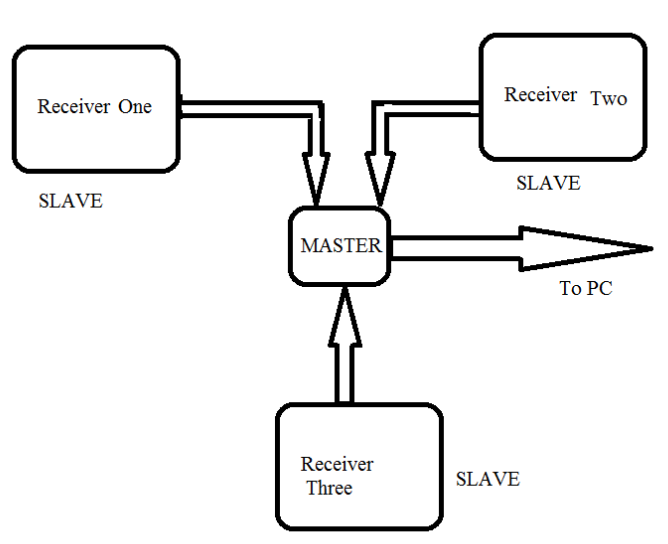
\includegraphics[width=120mm]{Images/MasterSlave.png}
	\caption{Data Collection Section Block Diagram}
	\label{fig:MasterSlave}
\end{figure}


\subsubsection{Communication Between Microcontrollers}
The output of tone decoder is either a logic high or a logic low. Logic high means the receiver is not receiving the required signal and logic low means that receiver is receiving required transmitted $40kHz$ ultrasonic signal.

The output of the tone decoder is fed into one of the $I/O$ pin of microcontroller ATMega8. Similarly, we have output of TSOP fed into another pin of the same microcontroller. The difference between time of arrival of the infrared signal, which is denoted by the output of TSOP and that of ultrasonic signal, which is denoted by the output of tone decoder is used for finding the distance between transmitter and receiver. All the calculations are performed within the microcontroller and thus the microcontroller contains the information of distance between transmitter and receiver.

In this way, all three microcontrollers residing on receiving modules comprise the information of distance between respective transmitters and receivers. All these distances are essential to determine the location of the transmitter using trilateration. As explained on the methodology section, when the distances between the transmitter and three predefined receivers are known, the location of a transmitter can be determined using trilateration.

This task of communicating between the microcontrollers is achieved by using \gls{spi}. \gls{spi} is one of the most used serial communication protocols.The \gls{spi} allows high-speed synchronous data transfer between the AVR and peripheral devices or between several AVR devices. The interconnection between two \gls{spi} devices always happens between a master device and a slave device. Compared to some peripheral devices like sensors which can only run in slave mode, the \gls{spi} of the AVR can be configured for both master and slave mode. The mode the AVR is running in is specified by the settings of the master bit (MSTR) in the \gls{spi} control register (SPCR). Special considerations about the SS pin have to be taken into account. This will be described later in the section “Multi Slave Systems - SS pin Functionality” on page 3. The master is the active part in this system and has to provide the clock signal a serial data transmission is based on. The slave is not capable of generating the clock signal and thus can not get active on its own. The slave just sends and receives data if the master generates the necessary clock signal. The master however generates the clock signal only while sending data. That means that the master has to send data to the slave to read data from the slave.

\subsubsection{Data Transmission Between Master and Slave}
The interaction between a master and a slave AVR is shown in Figure \ref{fig:Interaction}. Two identical SPI units are displayed. The left unit is configured as master while the right unit is configured as slave. The MISO, MOSI and SCK lines are connected with the corresponding lines of the other part. The mode in which a part is running determines if they are input or output signal lines. Because a bit is shifted from the master to the slave and from the slave to the master simultaneously in one clock cycle both 8-bit shift registers can be considered as one 16-bit circular shift register. This means that after eight SCK clock pulses the data between master and slave will be exchanged.
\begin{figure}[htpb]
	\centering
	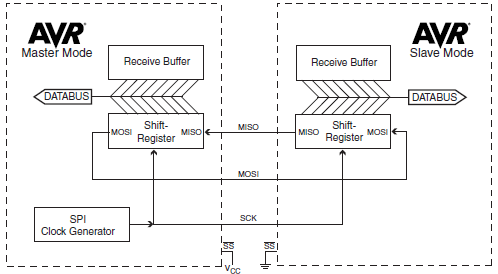
\includegraphics[scale=0.85]{Images/MasterandSlave.png}
	\caption{Interaction between a master and a slave}
	\label{fig:Interaction}
\end{figure}

The system is single buffered in the transmit direction and double buffered in the receive direction. This influences the data handling in the following ways:

\begin{enumerate}
	\item New bytes to be sent can not be written to the data register (SPDR) / shift register before the entire shift cycle is completed.
	\item Received bytes are written to the Receive Buffer immediately after the transmission is completed.
	\item The Receive Buffer has to be read before the next transmission is completed or data will be lost.
	\item Reading the SPDR will return the data of the Receive Buffer.
\end{enumerate}

After a transfer is completed the SPI Interrupt Flag (SPIF) will be set in the SPI Status Register (SPSR). This will cause the corresponding interrupt to be executed if this interrupt and the global interrupts are enabled. Setting the SPI Interrupt Enable (SPIE) bit in the SPCR enables the interrupt of the SPI while setting the I bit in the SREG enables the global interrupts.

\subsubsection{Pins of The SPI}
The SPI consists of four different signal lines. These lines are the shift clock (SCK), the Master Out Slave In line (MOSI), the Master In Slave Out line (MISO) and the active low Slave Select 3 line (SS). When the SPI is enabled, the data direction of the MOSI, MISO, SCK and SS pins are overridden according to the table.
\begin{table}[htpb]
\centering
\caption{SPI pin overrides}
\label{tab:Pinoverrides}
\begin{tabular}{|c|c|c|}
\hline 
Pin & Direction Master Mode & Direction Slave Mode \\ 
\hline 
MOSI & User Defined & Input \\ 
\hline 
MISO & Input & User Defined \\ 
\hline 
SCk & User Defined & Input \\ 
\hline 
$\overline{SS}$ & User Defined & Input \\ 
\hline 
\end{tabular} 
\end{table}

\subsubsection{Multi-Slave System}
The Slave Select $\overline{SS}$ pin plays a central role in the SPI configuration. Depending on the mode the part is running in and the configuration of this pin, it can be used to activate or deactivate the devices. The $\overline{SS}$ pin can be compared with a chip select pin which has some extra features. In master mode, the $\overline{SS}$ pin must be held high to ensure master SPI operation if this pin is configured as an input pin. A low level will switch the SPI into slave mode.

The ability to connect several devices to the same SPI-bus is based on the fact that only one master and only one slave is active at the same time. The multi-slave system is demonstrated by Figure \ref{fig:Multislave}.

\begin{figure}[htpb]
	\centering
	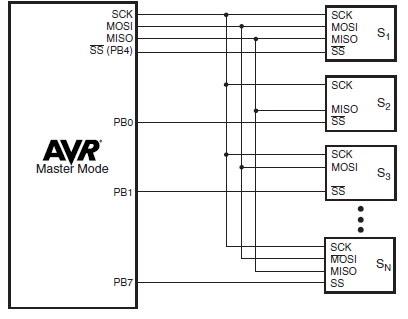
\includegraphics[scale=1]{Images/Multislave.png}
	\caption{Multi-Slave System}
	\label{fig:Multislave}
\end{figure}
Thus, the slave select pin of the slave whose data is to be transmitted to the master is held low at a time while the slave select pins of other slaves are held high. Thus, the master also knows from which slave it is receiving the data.

Thus, all three distances need to be fed into one another computational device for determining the location of the transmitter. Thus, all three microcontrollers send the information of distance into one another microcontroller, which feeds the data to PC via \gls{usb} cable where the task of locating the transmitter is done.

